\section{Lab 2}
\label{sec:lab2}
For the second part of the lab the task is to parallelize a serial implementation of the Red-Back Gauss-Seidal algorithm. This is done using OpenMP (Open \textbf Multi-\textbf Processing) which is an API for forming multi-threaded programs in C, C++, and Fortran. This parallel version is evaluated using the same simulator and CCPs as in \nameref{sec:lab1}. 

\subsection{Task 1}
The program first reads a matrix on the form $n \times n$ containing data points from a file. To make the program simpler and avoid special cases padding is added changing it's dimensions to $(n+2) \times (n+2)$. Then every other data point, here by called red dots, is looped through. For every red dot, an average of itself and it's neighbors to the west, south, north, and east is calculated and written as the dot's new value. The same procedure is performed on all the other data points, called black dots. The distribution of the red and black dots forms a chess pattern. This means that when the average for a dot and it's neighbors is calculated, all the neighbors are of the other color. The difference of the dots new and old values is added together and the process of calculating new averages is repeated until this accumulated difference of averages, divided by $n^2$, is smaller than $0.01$. When the program finishes the matrix have converged to an average of all red and black dots.

\subsection{Task 2}
\label{subsec:lab2:task2}
In listing~\ref{lst:solve} a parallelized version of the function \texttt{void Solve(double **A)} is shown. The approach taken to parallelize the function is to distribute the rows of the matrix evenly between all threads. This is done twice, once for the red dots and once for the black dots. Only one thread resets \texttt{diff} to zero on line 5 and test whether the program is finished or not on line 25. At each for loop that goes through the red and black dots the directive \texttt{reduction(+:diff)} is used which causes each thread to have its own private version of \texttt{diff} that gets added together after the for loop.

\subsection{Task 3}
To be able to evaluate the program described in \nameref{subsec:lab2:task2}, we decide to mimic the working set sizes in \nameref{sec:lab1}. However, the provided data files does not include a matrix big enough to fill neither each threads L1 cache or the LLC cache and thus is it expected that the results will not differentiate to a high degree by using the various working sets. 

In \reffig{fig:lab2}, results from running the parallelized version of the program in the simulator with different CCPs and different matrix dimensions are shown. It can be seen that using MESI over MSI does not cause any noticeable increase in performance. The data elements are mostly in the M state, which makes that the benefit of MESI's E state is low. The benefit is shown in Table~\ref{tbl:lab2}, where the number of \textit{WriteMisses} and \textit{InvalidationsSent} are a bit lower for MESI than MSI and the gap becomes bigger as the matrix size increases. This does not show in \reffig{fig:lab2}, as the cycle count is not dominated by \textit{WriteMisses} and \textit{InvalidationsSent}.

To use MESI-MG instead of MESI or MSI yields a huge performance degradation of 420\%, 394\%, and 430\% for matrix size 25, 100, and 200, respectively. This is because the sharing performed of the brim rows between threads. For each read of a dot in any of these rows, the dot is migrated to the reading thread. The frequent migration of dots generates a large number of \textit{ReadMissesSerivcedByModfied}, as can be seen in Table~\ref{tbl:lab2}. The overhead stays fairly constant compared to the other CCPs when the matrix size increases. This is due to the proportion of sharing between the threads stays the same.  

\begin{figure}[t]
	\center
	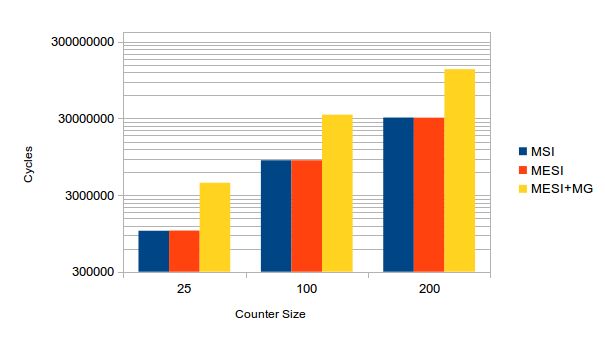
\includegraphics[width=0.8\textwidth]{lab2bars}
	\caption{Results from simulation of the parallelized benchmark for all cache coherence protocols combined with different working sets.}
	\label{fig:lab2}
\end{figure}

\subsection{Task 4}
To add the Owner (O) state to the existing MESI CCP, only small changes are needed. In \textit{readLine()} and \textit{remoteWriteAction()} no changes are needed. Turning to \textit{readRemoteAction()}, transitions from the E, M, and O states to the O state are added, and all of these transitions provide data to the calling cache. The action taken when in the shared state is removed. For \textit{writeLine()}, the only change needed is to take the same actions as when in the O state as in the S state. For the cache access statistics there is no need for change.

\par\noindent
\begin{minipage}[t]{.5\textwidth}
\begin{lstlisting}[language=C,frame=lrtb]
In readLine()
	if(MODIFIED) {...}
	if(EXCLUSIVE) {...}

	if(SHARED)
		return data		

In writeRemoteAction()
	if(SHARED) {...}
\end{lstlisting}%
\end{minipage}%
\hfill
\begin{minipage}[t]{.5\textwidth}
\begin{lstlisting}[frame=lrtb]
In readLine()
	if(MODIFIED || EXCLUSIVE || OWNER) 
		state = OWNER
		return data

	if(SHARED)
	{}

In writeRemoteAction()
	if(SHARED || OWNER) {...}
\end{lstlisting}%
\end{minipage}%
